\documentclass[10pt, twoside, openany]{book}

\usepackage[a4paper, top=2.5cm, bottom=2.5cm, left=3cm, right=3cm]{geometry}
\usepackage[utf8]{inputenc}
\usepackage[italian]{babel}
\usepackage{cite}
\usepackage[numbers, sort&compress]{natbib}
\usepackage{hyperref}
\usepackage{graphicx}
\usepackage{fancyhdr}
\usepackage[Lenny]{fncychap}
\usepackage{frontespizio}

\pagestyle{fancy}
\fancyhead{}
\fancyhead[LE]{\rightmark\hfill\leftmark}
\fancyhead[RO]{\leftmark\hfill\rightmark}
\bibliographystyle{unsrtnat}

\begin{document}
\begin{frontespizio}
\Universita{Roma Tor Vergata}
\Dipartimento{Ingegneria Civile e Ingegneria dell'Informazione}
\Corso{Ingegneria Informatica}
\Annoaccademico{2023/2024}
\Titolo{Titolo della tesi}
\Candidato[0316179]{Matteo Fanfarillo}
\Relatore{Giuseppe Bianchi}
\Correlatore{Francesco Gringoli}
\Logo{logo.png}
\end{frontespizio}

\begin{flushright}
\null\vspace{\stretch{1}}
\textit{[Citazione]}
\vspace{\stretch{2}}\null
\end{flushright}

\tableofcontents
\listoffigures
\listoftables

\chapter{Introduzione}
\section{Panoramica sulla eSIM}
La eSIM (embedded-SIM) non è altro che una SIM virtuale: grazie a lei, quando l'utente vuole cambiare operatore, non deve più acquistare fisicamente una nuova SIM card presso un negozio del nuovo operatore, bensì gli è sufficiente ricevere via e-mail un profilo, ossia una "SIM digitale" che può essere caricata subito sul telefono mediante la scansione di un QR code. Si tratta di una soluzione molto più pratica rispetto a recarsi fisicamente presso il negozio dell'operatore, tant'è vero che negli ultimi anni si sta diffondendo sempre di più: uno studio di Juniper Research stima che il numero di telefoni che utilizzano la connettività eSIM aumenterà dai 986 milioni attuali ai 3.5 miliardi entro il 2027 \cite{Corcom}. Per questi motivi, e poiché le informazioni associate alla comunicazione tra eSIM sono sensibili, è fondamentale garantire un livello di sicurezza sufficientemente elevato per il funzionamento della eSIM sia a run-time che a boot-time.

\section{Obiettivo del lavoro}
La presente trattazione si propone di effettuare un'analisi di sicurezza e delle vulnerabilità della eSIM e del suo funzionamento e, successivamente, di tentare di sfruttare, anche con delle attività di laboratorio, le eventuali vulnerabilità trovate.

\section{Definizioni preliminari}
\begin{itemize}
\item \textbf{eUICC (embedded Universal Integrated Circuit Card)}: è un chip utilizzato all'interno dei telefoni all'interno del quale è embeddato il software della eSIM. È integrato direttamente nei dispositivi (i.e. non è rimovibile) ed è progettato per essere programmato a distanza. Può contenere uno o più profili eSIM.
\item \textbf{SM-DP+ (Subscription Manager Data Preparation plus)}: è un protocollo che rappresenta una tecnica di provisioning usata per configurare le eSIM in modo automatico e remoto. Rispetto alla versione base SM-DP, offre delle funzionalità aggiuntive come un sistema di crittografia più avanzato e un'architettura di rete più flessibile.
\item \textbf{LPA (Local Profile Assistant)}: è un'applicazione che vive nel telefono dell'utente ed è responsabile della gestione dei profili all'interno della rete mobile, incluse la creazione, l'aggiornamento e la cancellazione.
\end{itemize}

\section{Panoramica sui capitoli successivi}
Nel capitolo 2 verrà svolta una trattazione dettagliata sull'architettura e sulle interfacce della eSIM, con lo scopo di fornire al lettore gli strumenti per comprendere appieno le tematiche centrali del lavoro. Nel capitolo 3 verrà effettuata un'analisi della sicurezza della eSIM a run-time, mentre nel capitolo 4 si procederà con l'analisi della sicurezza della eSIM a boot-time (i.e. durante la fase di configurazione).

\chapter{Interfacce e funzionamento della eSIM}
\section{Architettura di RSP}
Per comprendere appieno come funziona e come si interfaccia la eSIM all'interno dei dispositivi mobili, è necessario introdurre il protocollo RSP, anche perché la eSIM si colloca proprio all'interno dell'architettura di RSP.\\
RSP (Remote SIM Provisioning) è un protocollo utilizzato dal protocollo SM-DP+ per gestire la comunicazione tra il server SM-DP+ e la scheda eSIM del dispositivo mobile (i.e. l'eUICC). In particolare, definisce le operazioni di provisioning specifiche per la comunicazione dell'eUICC. Quest'ultimo comprende i dati sia dell'operatore che dell'utente che, nel caso delle SIM tradizionali, verrebbero appunto memorizzati su una SIM card fisica. Entrando più nel dettaglio sul funzionamento di RSP, l'end user che vuole ottenere un profilo eSIM offerto da un particolare operatore (nel quale viene definito un piano tariffario), deve pagare l'operatore affinché esso gli fornisca un codice QR. Dopodiché, deve effettuare la scansione di tale codice QR per avviare lo scaricamento (operazione di Download) e l'installazione (operazione di Install) del profilo eSIM: a questo punto, la connessione tra end user (col relativo profilo eSIM) e operatore è completata. Se in un secondo momento l'end user ha la necessità di ottenere e utilizzare un secondo profilo eSIM, gli è sufficiente ripetere i medesimi passaggi appena descritto, e questo secondo profilo può essere installato all'interno del medesimo eUICC che ospita già il primo profilo. Tale meccanismo è illustrato nella figura \ref{fig:RSP-functioning} tratta da \cite{GSMA-whitepaper}.
\begin{figure}
  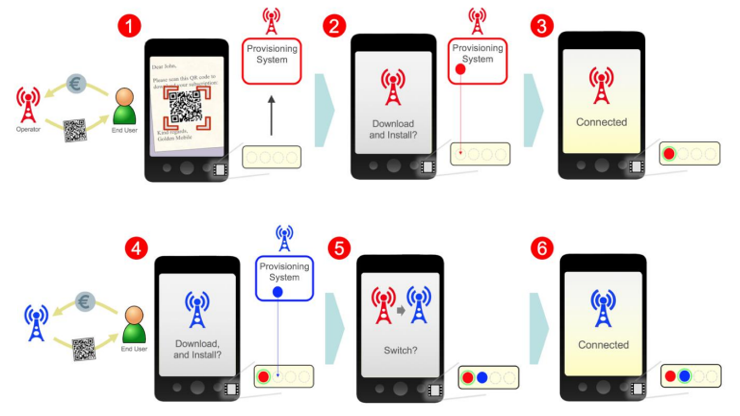
\includegraphics[width=\linewidth]{RSP-functioning.png}
  \caption{Comunicazione tra end user e operatore nel contesto del Remote SIM Provisioning.}
  \label{fig:RSP-functioning}
\end{figure}
\\Per quanto riguarda l'architettura interna di RSP nello specifico, esistono due soluzioni differenti \cite{GSMA-docs}.

\chapter{Analisi della sicurezza della eSIM a run-time}
[TODO]

\chapter{Analisi della sicurezza della eSIM a boot-time}
\section{Funzionamento del boot della eSIM}
[TODO]

\section{Potenziali vulnerabilità}
[TODO]

\section{Prove sperimentali}
[TODO]

\chapter{Conclusione}
[TODO]
\cite{Android-docs}

\bibliography{Bibliography}

\chapter*{Ringraziamenti}
[TODO]

%\begin{figure}
%  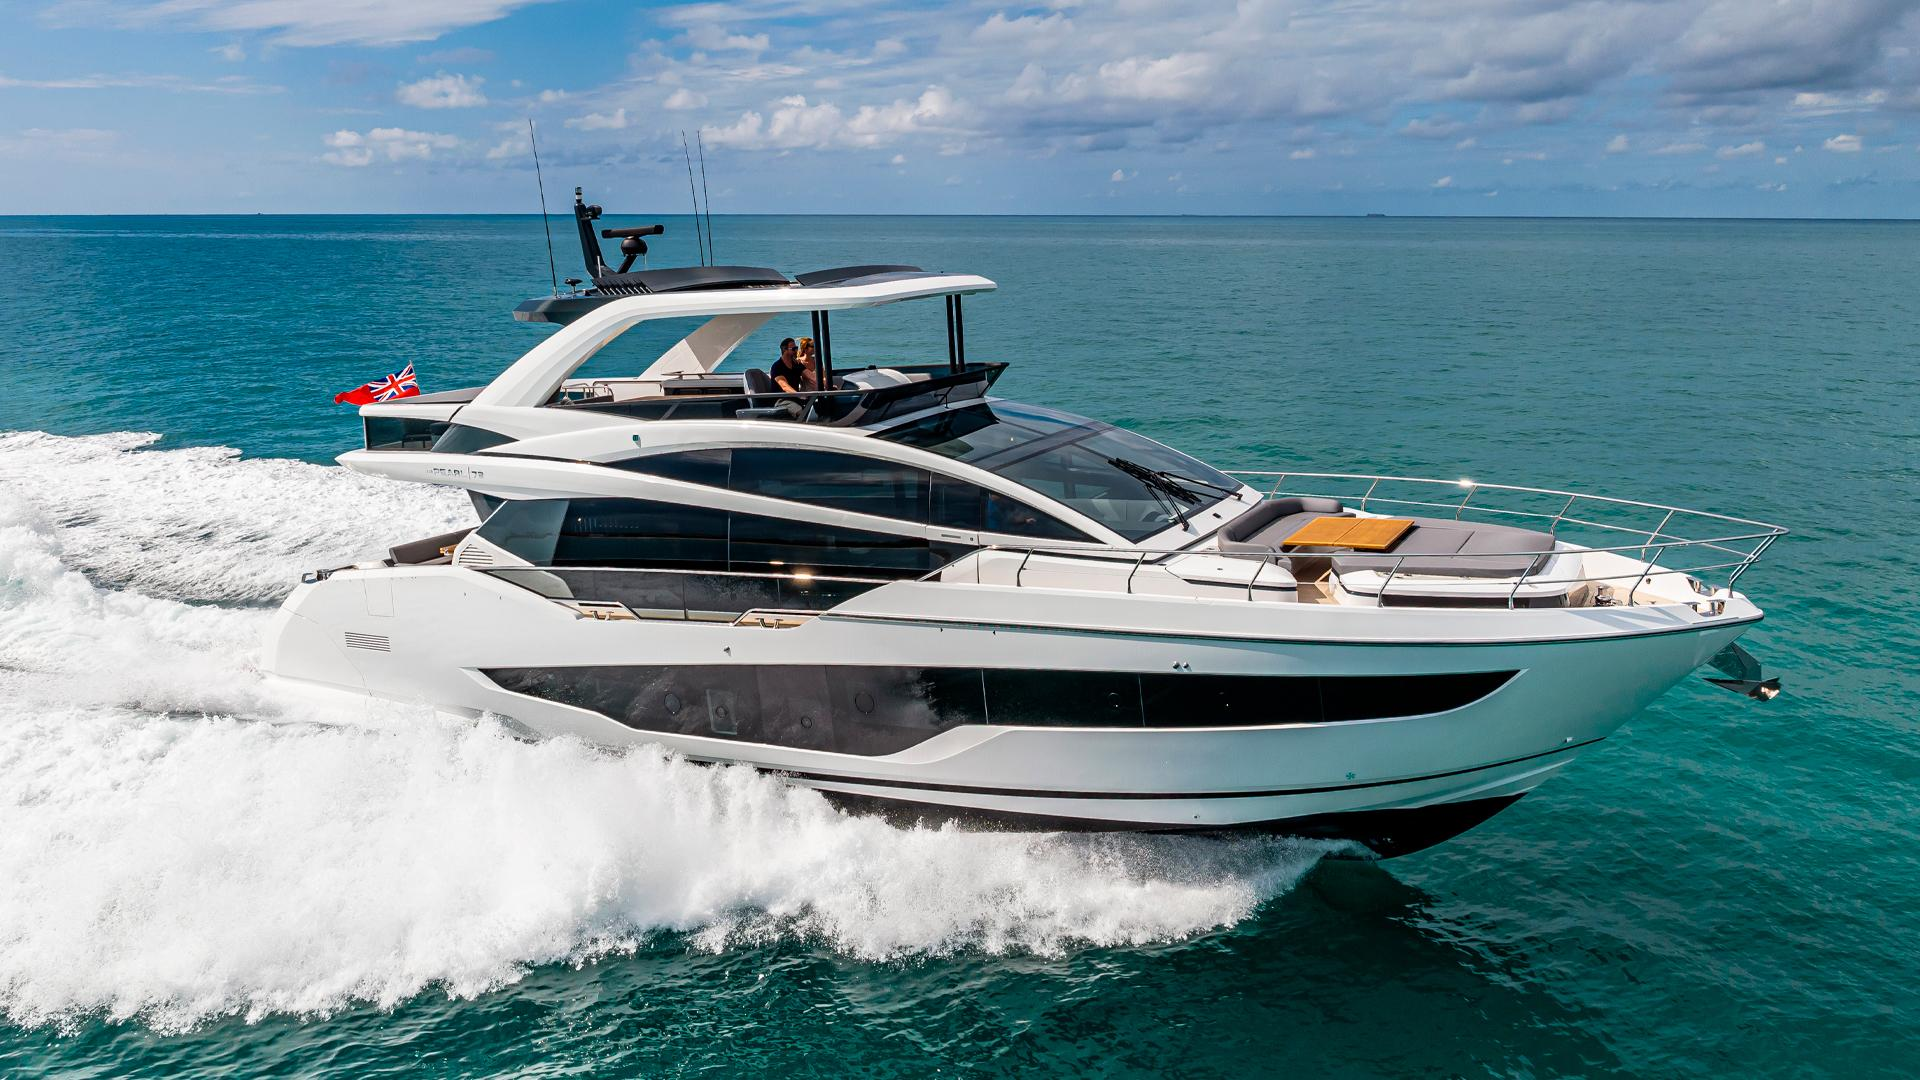
\includegraphics[width=\linewidth]{boat.jpeg}
%  \caption{A boat.}
%  \label{fig:boat1}
%\end{figure}
%Figure \ref{fig:boat1} shows a boat.

%\begin{table}[h!]
%  \begin{center}
%    \caption{Your first table.}
%    \label{tab:table1}
%    \begin{tabular}{l|c|r} % <-- Alignments: 1st column left, 2nd middle and 3rd right, with vertical lines in between
%      \textbf{Value 1} & \textbf{Value 2} & \textbf{Value 3}\\
%      $\alpha$ & $\beta$ & $\gamma$ \\
%      \hline
%      1 & 1110.1 & a\\
%      2 & 10.1 & b\\
%      3 & 23.113231 & c\\
%    \end{tabular}
%  \end{center}
%\end{table}

\end{document}